\documentclass[12pt,letterpaper]{article}
\usepackage{graphicx,textcomp}
\usepackage{natbib}
\usepackage{setspace}
\usepackage{fullpage}
\usepackage{color}
\usepackage[reqno]{amsmath}
\usepackage{amsthm}
\usepackage{fancyvrb}
\usepackage{amssymb,enumerate}
\usepackage[all]{xy}
\usepackage{endnotes}
\usepackage{lscape}
\newtheorem{com}{Comment}
\usepackage{float}
\usepackage{hyperref}
\newtheorem{lem} {Lemma}
\newtheorem{prop}{Proposition}
\newtheorem{thm}{Theorem}
\newtheorem{defn}{Definition}
\newtheorem{cor}{Corollary}
\newtheorem{obs}{Observation}
\usepackage[compact]{titlesec}
\usepackage{dcolumn}
\usepackage{tikz}
\usetikzlibrary{arrows}
\usepackage{multirow}
\usepackage{xcolor}
\newcolumntype{.}{D{.}{.}{-1}}
\newcolumntype{d}[1]{D{.}{.}{#1}}
\definecolor{light-gray}{gray}{0.65}
\usepackage{url}
\usepackage{listings}
\usepackage{color}

\definecolor{codegreen}{rgb}{0,0.6,0}
\definecolor{codegray}{rgb}{0.5,0.5,0.5}
\definecolor{codepurple}{rgb}{0.58,0,0.82}
\definecolor{backcolour}{rgb}{0.95,0.95,0.92}

\lstdefinestyle{mystyle}{
	backgroundcolor=\color{backcolour},   
	commentstyle=\color{codegreen},
	keywordstyle=\color{magenta},
	numberstyle=\tiny\color{codegray},
	stringstyle=\color{codepurple},
	basicstyle=\footnotesize,
	breakatwhitespace=false,         
	breaklines=true,                 
	captionpos=b,                    
	keepspaces=true,                 
	numbers=left,                    
	numbersep=5pt,                  
	showspaces=false,                
	showstringspaces=false,
	showtabs=false,                  
	tabsize=2
}
\lstset{style=mystyle}
\newcommand{\Sref}[1]{Section~\ref{#1}}
\newtheorem{hyp}{Hypothesis}

\title{Problem Set 2 Answers}
\date{\today}
\author{Kaley Burg}


\begin{document}
	\maketitle
	\section*{Note}
		Please note that the R file used in this tex file is \texttt{PS02\_answers\_KB\_Cleaned\_R.R} because that was the simplified version of my script. However, the mistakes, previous tries, and the code I used to come up with my for loops is in another R script called \texttt{PS02\_R\_KB\_safety.R}
		 and this is also in my Github. 
	\section*{Instructions}
\begin{itemize}
	\item Please show your work! You may lose points by simply writing in the answer. If the problem requires you to execute commands in \texttt{R}, please include the code you used to get your answers. Please also include the \texttt{.R} file that contains your code. If you are not sure if work needs to be shown for a particular problem, please ask.
	\item Your homework should be submitted electronically on GitHub.
	\item This problem set is due before 23:59 on Sunday October 15, 2023. No late assignments will be accepted.

\end{itemize}

	
	\vspace{.5cm}
	\section*{Question 1: Political Science}
		\vspace{.25cm}
	The following table was created using the data from a study run in a major Latin American city.\footnote{Fried, Lagunes, and Venkataramani (2010). ``Corruption and Inequality at the Crossroad: A Multimethod Study of Bribery and Discrimination in Latin America. \textit{Latin American Research Review}. 45 (1): 76-97.} As part of the experimental treatment in the study, one employee of the research team was chosen to make illegal left turns across traffic to draw the attention of the police officers on shift. Two employee drivers were upper class, two were lower class drivers, and the identity of the driver was randomly assigned per encounter. The researchers were interested in whether officers were more or less likely to solicit a bribe from drivers depending on their class (officers use phrases like, ``We can solve this the easy way'' to draw a bribe). The table below shows the resulting data.

\newpage
\begin{table}[h!]
	\centering
	\begin{tabular}{l | c c c }
		& Not Stopped & Bribe requested & Stopped/given warning \\
		\\[-1.8ex] 
		\hline \\[-1.8ex]
		Upper class & 14 & 6 & 7 \\
		Lower class & 7 & 7 & 1 \\
		\hline
	\end{tabular}
\end{table}

\begin{enumerate}
	
	\item [(a)]
	Calculate the $\chi^2$ test statistic by hand/manually (even better if you can do "by hand" in \texttt{R}).\\
%	\vspace{0cm}
	
		\begin{itemize}
			\item First I created a matrix with the data that was given, with 2 rows and 3 columns. I put this in a variable named polscidata. Then I added row and column names to correspond with what was provided. This code is given here:
				\lstinputlisting[language=R, firstline=33, lastline=35]{PS02_answers_KB_Cleaned_R.R}  
			\item Then I made a table with the conditional proportions of the table (in other words, a table with the probabilities of two specific values of each of the variables co-occurring together). This was not necessary to the analysis, but I looked at it regardless. The code is as follows:
				\lstinputlisting[language=R, firstline=39, lastline=39]{PS02_answers_KB_Cleaned_R.R}
			\item Then I made a table with the sums of the rows and columns and saved it in a new variable. This was mostly to check my work in the later steps
				\lstinputlisting[language=R, firstline=45, lastline=45]{PS02_answers_KB_Cleaned_R.R}
			\item Then I made a new matrix to fill with expected values. I also made the column and row names the same as the previous matrix
				\lstinputlisting[language=R, firstline=61, lastline=63]{PS02_answers_KB_Cleaned_R.R}
			\item For the actual "by hand" computation in R, I created a for loop that iterated through value of the matrix "polscidata". For each value, the loop saved the row sums, column sums, and total sum and computed a new value corresponding to the formula: (row sum/total sum)*column sum. Lastly, I added this to the empty matrix ("expected") that I made earlier
				\lstinputlisting[language=R, firstline=77, lastline=84]{PS02_answers_KB_Cleaned_R.R}
			\item Then, for clarity, I decided to change the name of my variable "polscidata" to "observed" as this aligns with the further computation
				\lstinputlisting[language=R, firstline=89, lastline=89]{PS02_answers_KB_Cleaned_R.R}
			\item Next, I made a new variable "X2" to represent my test statistic. This variable is created to correspond with 0, allowing me to use it in a for loop. I then made a for loop that iterates through my matrices and sums together the observed values minus the expected values, squares this value, and then divides it by the expected values. $\sum \left(\frac{(f_{\text{observed}} - f_{\text{expected}})^2}{f_{\text{expected}}}\right)
			$ Then, after each iteration, it adds this value to my X2 variable, such that X2 ends up being the total sum. X2 then holds the value of my test statistic. The code is as follows:
				\lstinputlisting[language=R, firstline=101, lastline=105]{PS02_answers_KB_Cleaned_R.R}
			\item The code returns a value of \textbf{3.791168}. This is our test statistic
		\end{itemize}
	
	\item [(b)]
	Now calculate the p-value from the test statistic you just created (in \texttt{R}).\footnote{Remember frequency should be $>$ 5 for all cells, but let's calculate the p-value here anyway.}  What do you conclude if $\alpha = 0.1$?\\
	
		\begin{itemize}
			\item To find the p-value, I used code from class. First I made a degrees of freedom variable, then made a new object "pvalue" using the pchisq function:
				\lstinputlisting[language=R, firstline=119, lastline=119]{PS02_answers_KB_Cleaned_R.R}
				\lstinputlisting[language=R, firstline=125, lastline=125]{PS02_answers_KB_Cleaned_R.R}
			\item If alpha = 0.1, we fail to reject the null hypothesis because our p value of \textbf{0.1502306} is greater than the alpha value of 0.1. What this means is that we fail to reject the null hypothesis that solicitation of bribe and class are independent of each other.
		\end{itemize}
	  	
	
	\newpage
	\item [(c)] Calculate the standardized residuals for each cell and put them in the table below.
	\vspace{1cm}
	
	\begin{table}[h]
		\centering
			\begin{tabular} {l | c c c }
			& Not Stopped & Bribe requested & Stopped/given warning \\
			\\[-1.8ex] 
			\hline \\[-1.8ex]
			Upper class & 0.3220306 & -1.641957  & 1.523026 \\
			Lower class & -0.3220306 & 1.641957 & -1.523026 \\
			\hline
			\end{tabular}
	\end{table}
	
		\begin{itemize}
			\item  For this, we know that the numerator of the formula of standardized residuals is ok so the numerator of the equation is $f_{expected} - f_{observed}$, so I made a new matrix called "unstandresid with these values using this code:
				\lstinputlisting[language=R, firstline=146, lastline=146]{PS02_answers_KB_Cleaned_R.R}
			\item I then changed the name to "numerator" for the sake of the computation
				\lstinputlisting[language=R, firstline=148, lastline=148]{PS02_answers_KB_Cleaned_R.R}
			\item Next, I made an empty matrix called denominator. Then, I combined the old for loop that I used to get the expected values to fill the matrix with denominators following this formula for the denominator: $\sqrt{f_{\text{expected}}(1 - \text{row prop.})(1 - \text{column prop.})}$ This code is as follows:
				\lstinputlisting[language=R, firstline=151, lastline=153]{PS02_answers_KB_Cleaned_R.R}
				\lstinputlisting[language=R, firstline=157, lastline=166]{PS02_answers_KB_Cleaned_R.R}
			\item This then gave me 2 matrices, 1 with the numerators and another with the denominators. This allowed me to put them together into a new matrix by dividing "numerator" by "denominator". I did this in the creation of a new matrix "stdresids"
				\lstinputlisting[language=R, firstline=175, lastline=175]{PS02_answers_KB_Cleaned_R.R}
			\item I then checked these values with the chisq.test function and I get the same results
				\lstinputlisting[language=R, firstline=180, lastline=181]{PS02_answers_KB_Cleaned_R.R}
				
		\end{itemize}
		
		
	\vspace{0cm}
	\item [(d)] How might the standardized residuals help you interpret the results?  
		\begin{itemize}
			\item A residual is the difference between an observed and expected cell frequency. The residual is positive when the observed frequency exceeds the expected value under the null hypothesis. The residual is negative when the observed frequency is smaller than the expected value. The standardized residuals describe the pattern of the association among the cells. A large standardized residual provides evidence against independence (the null hypothesis) in that cell. Values below -3 or above +3 are strong evidence against independence in the given cell (Agresti and Finlay (p. 230)).
			\item In this case, none of the standardized residuals exceed -3 or +3, so we can conclude that there is no overly strong evidence against independence in any given cell. However, we can conclude that the cells corresponding to "bribe requested" and "class" as well as the cells corresponding to "stopped/given warning" and "class" are most significantly than what would be expected under the null hypothesis.
			\item In other words, bribes were requested less often for those of upper class and more often for those of lower class than would be expected if class and solicitation are said to be independent.
				\begin{itemize}
					\item This is the most useful for determining the initial research question of whether officers were more or less likely to solicit a bribe from drivers depending on their class
				\end{itemize}
			\item Furthermore, participants were stopped/given a warning more often for those of upper class and less often for those of lower class than would be expected if class and solicitation are said to be independent.
			\item Lastly, participants were not stopped more often for those of upper class and less often for those of lower class than would be expected if class and solicitation are said to be independent
			\item These residuals and their interpretation can help us interpret our results by allowing us to see that bribe solicitation seems to be influenced by class (note: I am saying influenced by as this is an experimental study with randomized controls, meaning that the language surrounding it can go beyond pure association). Particularly, we see the highest deviation from what would be expected under the null hypothesis in the "bribe requested" category, specifically that bribes were requested from those of lower class standing than would be expected under the null hypothesis. From this we can assume that those of police officers are more likely to solicit a bribe from someone who is of a lower class standing.
		\end{itemize}
	
\end{enumerate}
\newpage

\section*{Question 2: Economics}
Chattopadhyay and Duflo were interested in whether women promote different policies than men.\footnote{Chattopadhyay and Duflo. (2004). ``Women as Policy Makers: Evidence from a Randomized Policy Experiment in India. \textit{Econometrica}. 72 (5), 1409-1443.} Answering this question with observational data is pretty difficult due to potential confounding problems (e.g. the districts that choose female politicians are likely to systematically differ in other aspects too). Hence, they exploit a randomized policy experiment in India, where since the mid-1990s, $\frac{1}{3}$ of village council heads have been randomly reserved for women. A subset of the data from West Bengal can be found at the following link: \url{https://raw.githubusercontent.com/kosukeimai/qss/master/PREDICTION/women.csv}\\

\noindent Each observation in the data set represents a village and there are two villages associated with one GP (i.e. a level of government is called "GP"). Figure~\ref{fig:women_desc} below shows the names and descriptions of the variables in the dataset. The authors hypothesize that female politicians are more likely to support policies female voters want. Researchers found that more women complain about the quality of drinking water than men. You need to estimate the effect of the reservation policy on the number of new or repaired drinking water facilities in the villages.
\vspace{.5cm}
\begin{figure}[h!]
	\caption{\footnotesize{Names and description of variables from Chattopadhyay and Duflo (2004).}}
	\vspace{.5cm}
	\centering
	\label{fig:women_desc}
	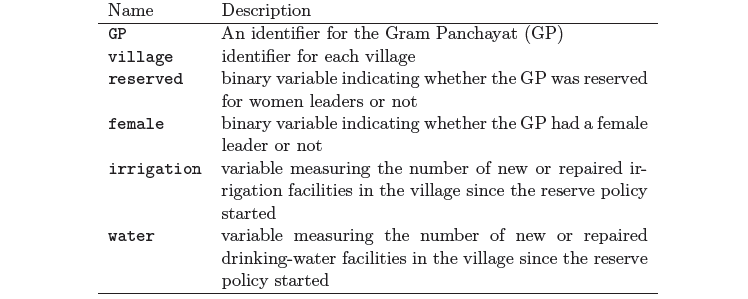
\includegraphics[width=1.1\textwidth]{women_desc.png}
\end{figure}		

\newpage
\begin{enumerate}
	\item [(a)] State a null and alternative (two-tailed) hypothesis. 
	
		\begin{itemize}
			\item Our linear model is $Y = \alpha + \beta X$, such that $\alpha$ is the Y-intercept, $\beta$ is the slope of the line, Y is the outcome vector and X is the vector of the predictor (as seen in the lecture slides)
			\item As this research question is looking at the effect of the reservation policy on the number of new or repaired drinking water facilities, it makes most sense to look at the coefficient ($\beta_1$). The hypotheses for such is (note: the lecture slides referred to $\beta$ as $\beta_1$ and $\alpha$ as $\beta_0$ so I will be using that notation in my hypotheses):
				\begin{itemize}
					\item {Null Hypothesis: $\beta_1$ $=$ 0}
					\item {Alternative Hypothesis: $\beta_1$ $\neq$ 0}
				\end{itemize}
			\item The null hypotheses for the intercept is as follows:
				\begin{itemize}
					\item {Null Hypothesis: $\beta_0$ $=$ 0}
					\item {Alternative Hypothesis: $\beta_0$ $\neq$ 0}
				\end{itemize}
		\end{itemize}
	
	\vspace{0cm}
	\item [(b)] Run a bivariate regression to test this hypothesis in \texttt{R} (include your code!).
			
		\begin{itemize}
			\item First I created a dataframe with the csv file provided. Then I plotted the reserved variable by the water variable. The question is asking whether the reservation policy (recorded in the reserved variable) has an effect on the number of new or repaired drinking water facilities (recorded in the water variable). I also plotted the regression line using the code for "model" in the next section of code.
				\lstinputlisting[language=R, firstline=191, lastline=191]{PS02_answers_KB_Cleaned_R.R}
				\lstinputlisting[language=R, firstline=220, lastline=225]{PS02_answers_KB_Cleaned_R.R}
				\includegraphics[width=.4\textwidth]{RegressionPlot}\hfill
			\item Next, I fit the linear regression model using the summary function. I did this two ways, as it was stated in tutorial that the latter way is better practice. Then I saved this model into an object named "model"
				\lstinputlisting[language=R, firstline=198, lastline=198]{PS02_answers_KB_Cleaned_R.R}
				\lstinputlisting[language=R, firstline=200, lastline=200]{PS02_answers_KB_Cleaned_R.R}
				\lstinputlisting[language=R, firstline=203, lastline=203]{PS02_answers_KB_Cleaned_R.R}
		\end{itemize}
			
			
	\vspace{0cm}
	\item [(c)] Interpret the coefficient estimate for reservation policy. 
		\begin{itemize}
			\item The value of $\beta_0$ is \textbf{14.738}
			\item The value of $\beta_1$ is \textbf{9.252}
			\item The coefficient estimate ($\beta_1$) is stating that an increase of 1 reservation policy is associated with an average increase in new or repaired drinking water facilities in the villages of 9.252. 
			\item However, this is not the best way to word this given that the reservation policy is coded as a binary variable. Rather, the change from no reservation policy to having a reservation policy is associated with an on average increase in new or repaired drinking water facilities in the villages of 9.252
				\begin{itemize}
					\item The p-value for this value is \textbf{0.0197}, so we can reject the null hypothesis at the 0.05 level.
				\end{itemize}
			\item Regarding $\beta_0$, the interpretion is: with no reservation policy, there is an average of 14.738 new or repaired drinking water facilities in the villages.
				\begin{itemize}
					\item The p-value for this value is \textbf{4.22e-10}, so we can reject the null hypothesis at the 0.001 level.
				\end{itemize}
			\item I think it is also important to note that this is a randomized experimental study, which also changes the interpretation of our results slightly. Under the assumption of causal inference, we would be able to say that \textbf{the reservation policy has an effect on the number of new or repaired drinking water facilities in the villages, such that the presence of a reservation policy causes an average increase of 9.25 new or repaired water facilities in the villages.}
			
		\end{itemize}
\end{enumerate}

\end{document}
